\chapter{Fundamentals and Related Work}
\label{chap:fundamentals}
%background - What do I need to know to understand the thesis?
This chapter provides the fundamental concepts and related work that are required to understand the presented approach discussed in Chapter\ref{chap:approach}.The first section introduces definitions of terms that are used throughout this document. The second section provides a brief introduction about the basic concepts of this thesis work.  The third and fourth sections present short description about  works related to the presented approach. The last section focuses on concepts of Resource-centric Organizational Modeling and its notations. Though modeling notations are not part of implementation, it has been introduced to assist the reader in better understanding. The last section also discusses about the process and entity representation of the organizational modeling.  



%%%%%%%%%%%%%%%%%%%%%%%%%%%%%%%%%%%%%%%%%%%%%%%%%%%%%%%%%%%%%%%%%%%%%%%%%
\section{Definitions of Terms}
\label{sec:termdefinitions}
%%%%%%%%%%%%%%%%%%%%%%%%%%%%%%%%%%%%%%%%%%%%%%%%%%%%%%%%%%%%%%%%%%%%%%%%%
\textit{Business Process} A business process has been defined as the set of activities and tasks whose final output is accomplishment of a goal.These activities are performed in an organizational and technical environment \cite{Weske2012}.  Based on the type of input and the operation of tasks, these processes can be categorized as management process, support process, research process, development process, etc. \cite{Sungur2015}     \\

\textit{Business Logic} Business logic refers to the activities that need to be done to execute the corresponding process. \\

\textit{Business Process Models} Business process models are models to capture recurring procedures during a business process execution and enact them in a automated fashion for re-using those stored knowledge. \\

\textit{Business Process Engines} Business process engines can enact the business process models automatically once the configuration of necessary infrastructure has been carried out \cite{Sungur2015}. \\

\textit{Business Process Management} Business process management (BPM) includes concepts, methods, and techniques to support the design, administration, configuration, enactment, and analysis of business processes \cite{Weske2012}. \\

\textit{Business Process Management Life Cycle} Business process management life cycle is the series of phases such as modeling, configuring, executing, and improving business process. These series phases are conducted as a cycle. \cite{Weske2012}\\

\textit{Informal Process}  The processes that human participate and create knowledge are called unstructured/informal/human-centric processes. In informal process, execution steps cannot be modeled or are not feasible to model before their enactments. This is because due to the dynamic changing behavior of execution steps of the informal processes.  For Example software development process is an informal process, where required activities and order of their execution cannot be determined beforehand \cite{Sungur2015}.       \\

\textit{Informal Process Essentials} Informal Process Essentials (IPE) is an intention-based approach that enables describing process declartively, i.e., without describing how the intention is achieved, and providing only information about what has to be achieved \cite{Sungur2014a}. \\

\textit{Autonomous Agents} Autonomous agents are those agents that enact informal processes based on the ad-hoc decisions, experience, and knowledge with the help of other involved resources   \cite{Sungur2015}. \\

\textit{Organizational Intentions} Intentions are defined hierarchically, which can contain and extend sub-intentions.It is depicted by a double circle. The sub-intentions are refined starting from main intentions. Intentions are associated with capabilities or resources. An accomplishment of an intention changes state. An intention can extend another intention.        \\

\textit{Organizational Resources} That drive towards the successful execution of the process. key for achieving specified process goals
In the context of our work, the definition of organizational resources refers not only the entities that are capable of doing work but also entities that have an impact on the outcome of the processes, e.g., software tools, human performers, data etc.      \\


\textit{Organizational Capabilities} Organizational capability is the ability to provide business values like software applications, resources, and potential of the actor to make decisions even in changing situations \cite{Stirna2012}.Describes a capability provided by a resource or required by an intention. The performers of an informal process have certain skills and roles to achieve the intention.   \\

\textit{Actors} Actors are type of organizational resources that drive execution of a process autonomously. Actors makes use of other resources as well to achieve \textit{intention} and \textit{sub-intention} of an informal process \cite{Sungur2015}.  \\




\textit{Strategies}         \\

%%%%%%%%%%%%%%%%%%%%%%%%%%%%%%%%%%%%%%%%%%%%%%%%%%%%%%%%%%%%%%%%%%%%%%%%%
\section{Basic Concepts}
\label{sec:basicconcepts}
%%%%%%%%%%%%%%%%%%%%%%%%%%%%%%%%%%%%%%%%%%%%%%%%%%%%%%%%%%%%%%%%%%%%%%%%%
Models are used in various fields like manufacturing, scientific, IT, etc.,. These models are mainly useful in re-using the predefined regular, intelligible and field-tested solutions. Such models has numerous benefits like performance improvement, reduced cost of operation and design, etc.,. Besides these processes there are processes which requires participation of human and performance of these  processes depend on human knowledge, i.e., they are subject to change and carried out based on experience of previous knowledge. These processes are called \textit{Informal Processes} and they do not have formal structured execution of steps for the enactment of processes. 

The work by Sungur et. al \cite{Sungur2014a} gives a comprehensive account of challenges in defining the business logic of informal processes as below:

\begin{itemize}
	\item The structure of informal processes are not known before enactment of the processes
	\item Results in less flexible and less efficient solutions
	\item The cost of creation of well-defined business logic is too high
\end{itemize}

%%%%%%%%%%%%%%%%%%%%%%%%%%%%%%%%%%%%%%%%%%%%%%%%%%%%%%%%%%%%%%%%%%%%%%%%%
\subsection{Informal Process Essentials}
\label{sec:informalprocessessentials}
%%%%%%%%%%%%%%%%%%%%%%%%%%%%%%%%%%%%%%%%%%%%%%%%%%%%%%%%%%%%%%%%%%%%%%%%%
In this section, we provide an overview about the concepts introduced in the approach Informal Process Essentials (IPE) \cite{Sungur2014a}. This thesis work realizes the concept of \textit{resource-centric modeling of informal processes}, specified in the above approach by Sungur et al.  As mentioned in the Section \ref{sec:termdefinitions}, resources are drivers to achieve intentions in the informal processes. In IPE approach, the author differentiates the resources based on the time the resources are needed in the informal processes as below :
  \begin{itemize}
  	\item \textit{Initial resources} which are required during the start of informal processes.
  	\item \textit{On-demand resources} that are required based on intentions during process enactment.
  	\item \textit{Actors} are the resources in IPE meta-model, that drive process execution autonomously.
  	\item \textit{Knowledge resources} resources that contain important information required for the enactment of a process. These are critical for guiding actors.  
  \end{itemize}
Informal Process Essentials (IPE) describes the following about informal process \cite{Sungur2014} 

\begin{itemize}
	\item Describes the constituents informal process such as performers, data and software tools
	\item Describes how to make core element ready for the enactment of the informal process i.e resource providers
\end{itemize}




%%%%%%%%%%%%%%%%%%%%%%%%%%%%%%%%%%%%%%%%%%%%%%%%%%%%%%%%%%%%%%%%%%%%%%%%%
\section{Human Centric Process}
\label{sec:humancentric}
%%%%%%%%%%%%%%%%%%%%%%%%%%%%%%%%%%%%%%%%%%%%%%%%%%%%%%%%%%%%%%%%%%%%%%%%%



%%%%%%%%%%%%%%%%%%%%%%%%%%%%%%%%%%%%%%%%%%%%%%%%%%%%%%%%%%%%%%%%%%%%%%%%%
\section{Second Phase of InProcXec}
\label{sec:inproxec}
%%%%%%%%%%%%%%%%%%%%%%%%%%%%%%%%%%%%%%%%%%%%%%%%%%%%%%%%%%%%%%%%%%%%%%%%%
In this section, we present the \textit{InProXec} method, proposed by Sungur et al. in \cite{Sungur2015}. Since this thesis work is realizing \textit{resource-centric informal process modeling} , the main focus of this section is on the second phase of InProXec. The method described in Figure \ref{fig:inprocxec_steps}, initializes informal process models in an automated fashion. In the following paragraphs, we present an overview of the method and overview about different phases of the method with a detailed overview about the second phase of the \textit{InProXec} method. 

\begin{figure}
	\centering
	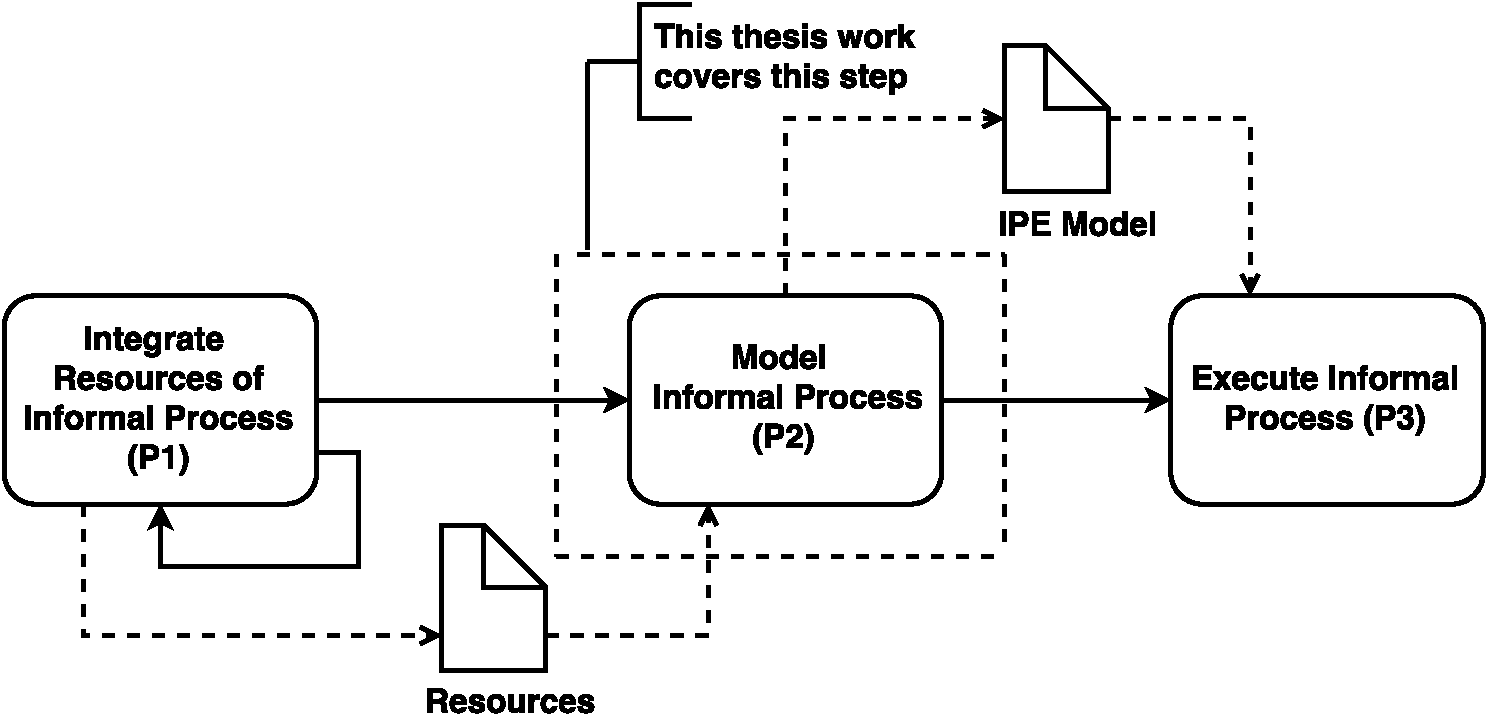
\includegraphics[width=\textwidth]{InProXec_Steps.pdf}
	\caption{Steps of InProXec method \cite{Sungur2015}}
	\label{fig:inprocxec_steps}
\end{figure} 

As shown in the Figure \ref{fig:inprocxec_steps}, the InProcXec method consists of four different phases.

\textit{Integrating Resources of Informal Processes (P1)} To model an informal process, we need information about the resources, these information are collected beforehand during process execution. There exist many services to acquire information about informal processes resources automatically. The final output of this phase is integrated resources which are required as an input to next modeling phase. Thus this phase sets up an environment required for modeling and execution of informal processes.  \\

\textit{Informal Process Modeling (P2)}  This phase receives the resource definitions made available in the first phase P1 as an input.  Based on this, business experts model informal processes using different IPE modeling elements. For example business experts create informal process models using resources aiming to achieve main intentions that contains sub-intentions.   \\

\textit{Informal Process Compilation (P3)}  Phase P2, describes only the intentions required to be achieved, corresponding required resources etc. But in phase P2, there is no facility to instantiate a functionality. Thus in third phase P3, the output of phase P2 is taken i.e IPE models and are transformed into intializable self-contained \textit{Deployable Informal Process Essentials Archives(DIPEA)} \cite{Sungur2015} takes place. This results in DIPEAs enacting required informal process. To realize, phase P3 an \textit{IPE Model COmpiler} also been introduced. \\

\textit{Informal Process Model Deployment and Runtime (P4)} This phase employs \textit{IPE Runtime} which parses DIPEAs and runs the executables contained in those archives. During this phase, the autonomous actors work towards intentions of informal processes using acquired resources and other involved resources.  \\


%%%%%%%%%%%%%%%%%%%%%%%%%%%%%%%%%%%%%%%%%%%%%%%%%%%%%%%%%%%%%%%%%%%%%%%%%
\subsection{Informal Process Modeling (P2)}
\label{subsec:informalprocessmodeling}
%%%%%%%%%%%%%%%%%%%%%%%%%%%%%%%%%%%%%%%%%%%%%%%%%%%%%%%%%%%%%%%%%%%%%%%%%

%%%%%%%%%%%%%%%%%%%%%%%%%%%%%%%%%%%%%%%%%%%%%%%%%%%%%%%%%%%%%%%%%%%%%%%%%
\section{Resource-centric Organizational Modeling}
%%%%%%%%%%%%%%%%%%%%%%%%%%%%%%%%%%%%%%%%%%%%%%%%%%%%%%%%%%%%%%%%%%%%%%%%%
 The Organizational Modeling element notation has been selected as per the guidelines mentioned in the paper by Daniel L.Moody \cite{Moody2009}. Also by observing  the fact that business process modelers are already well-known with the present process modeling notations such as Business Process Modeling Notation 2.0 (BPMN) \cite{bpm2011} and ArchiMate notation\cite{arc2013}, the shape depiction of organizational model elements are designed similar to those existing process notations. 

 Due to the importance of shapes in expressing the information visually , the notations are chosen in such a way that each element of Organizational Modeling  differ by shape. Also a legend will be always shown in the modeling notation to denote the meaning of each shape \cite{Moody2009}. As shape plays a primary role in discriminating between different element, organizational model notations are represented through individual shapes like rectangle, double circle, elliptic etc.,. The description of each element in the Organizational Model Notation is shown in the Table \ref{tab:notations}. 

\begin{center}
	\begin{longtable}{p{3cm}p{10cm}p{3cm}}
		\toprule 
		\textbf{Element} & \textbf{Definition} & \textbf{Notation} \\
		\midrule
		\endfirsthead
		Intentions 			& Intentions are purposeful concrete steps taken to achieve expected outcomes . They reflect the actual intention of an organization. & \begin{center} 
\includegraphics[width= 0.07\textwidth]{intentions.png}  \end{center}  \\  
		
		Capabilities	&  Capabilites are represented by a elliptical circle. Capability is an ability that should be possessed by an actor or a resource that work towards achievement of intention.   & \begin{center} 
\includegraphics[width= 0.1\textwidth]{capabilities.png} \end{center}   \\
		
		Context				& The environment that forms the setting for an event, statement, or idea, and in terms of which it can be fully understood. There are two Contexts: Initial and Final. The Initial Context is the situation which describes the driving forces that trigger the process to start. The Final Context is the expected situation once the process has finished.Both initial and final context are represented by an hexagonal shape except the final context has thick edges than initial context.  & \begin{center} 
\includegraphics[width= 0.1\textwidth]{context.png} \end{center}  \\
		
		
		Strategy		&  A method or plan chosen to bring about a desired future, such as accomplishment of a intention. Strategies are expressed by rectangles with sharp edges. In the conceptual Organizational Modeling, strategies are self-contained and loosely coupled elements.   & \begin{center} 
\includegraphics[width= 0.1\textwidth]{strategy.png} \end{center}   \\
		
		Resources					& The people and tools needed to fulfill the middle objectives or those/that work towards the achievement of goal . Resources are represented by a rounded rectangle. Resources are linked to capabilities and actors. & \begin{center} 
\includegraphics[width= 0.1\textwidth]{resources.png} \end{center}   \\
		
		Actors					& People who participate in the process. Actors are represented by a stick-man and they are linked to resource as actors can be resources. Actors define the strategy and goals.  & \begin{center} 
\includegraphics[width= 0.07\textwidth]{actor.png} \end{center}   \\
		
		Relationship				& A relationship is used specify the fixed links between the elements of the model. Relationship between two elements is represented by a single direction line which represents a sequence.  & \begin{center} 
\includegraphics[width= 0.1\textwidth]{relationship.png} \end{center}   \\
		
		
		\bottomrule
		\caption{Informal Process Modeling Notation}
		\label{tab:notations}		
	\end{longtable}	
\end{center}



%%%%%%%%%%%%%%%%%%%%%%%%%%%%%%%%%%%%%%%%%%%%%%%%%%%%%%%%%%%%%%%%%%%%%%%%%
\subsection{Process Representation}
%%%%%%%%%%%%%%%%%%%%%%%%%%%%%%%%%%%%%%%%%%%%%%%%%%%%%%%%%%%%%%%%%%%%%%%%%
Organizational Process Modeling depicted inFigure \ref{fig:processdiagram} captures required organizational capabilities that are satisfied by resource models  to enable the achievement of organizational goals in certain context definitions through a strategy. It is a top-down approach, i.e., first goals are defined and then sub-goals  are defined by refining main goal. Goals connect initial context definitions with final context definitions through a strategy.  To understand the definition of Organizational Process Modeling we need to interpret the Organizational Process Modeling Representation shown in Figure\ref{fig:processdiagram}. 

 The Organizational Process Modeling start with modeling of organizational goal (M1). Once the goal has been modeled, the second step is to model the strategies which can be a multi-instance strategy model(M2). The next step is to model the context definitions (M3.1), required organizational capabilities (M3.2) and refining the sub-goals from main goal in parallel. Once the required capabilities(M4) are matched by required resources(P1), modeling of resources(M5) can be done.  Based on created resource models (M5) and modeled context definitions(M3.1), strategies can be executed. The organizational goals would be iteratively updated supported to strategy execution.  


\begin{figure}
	\centering
	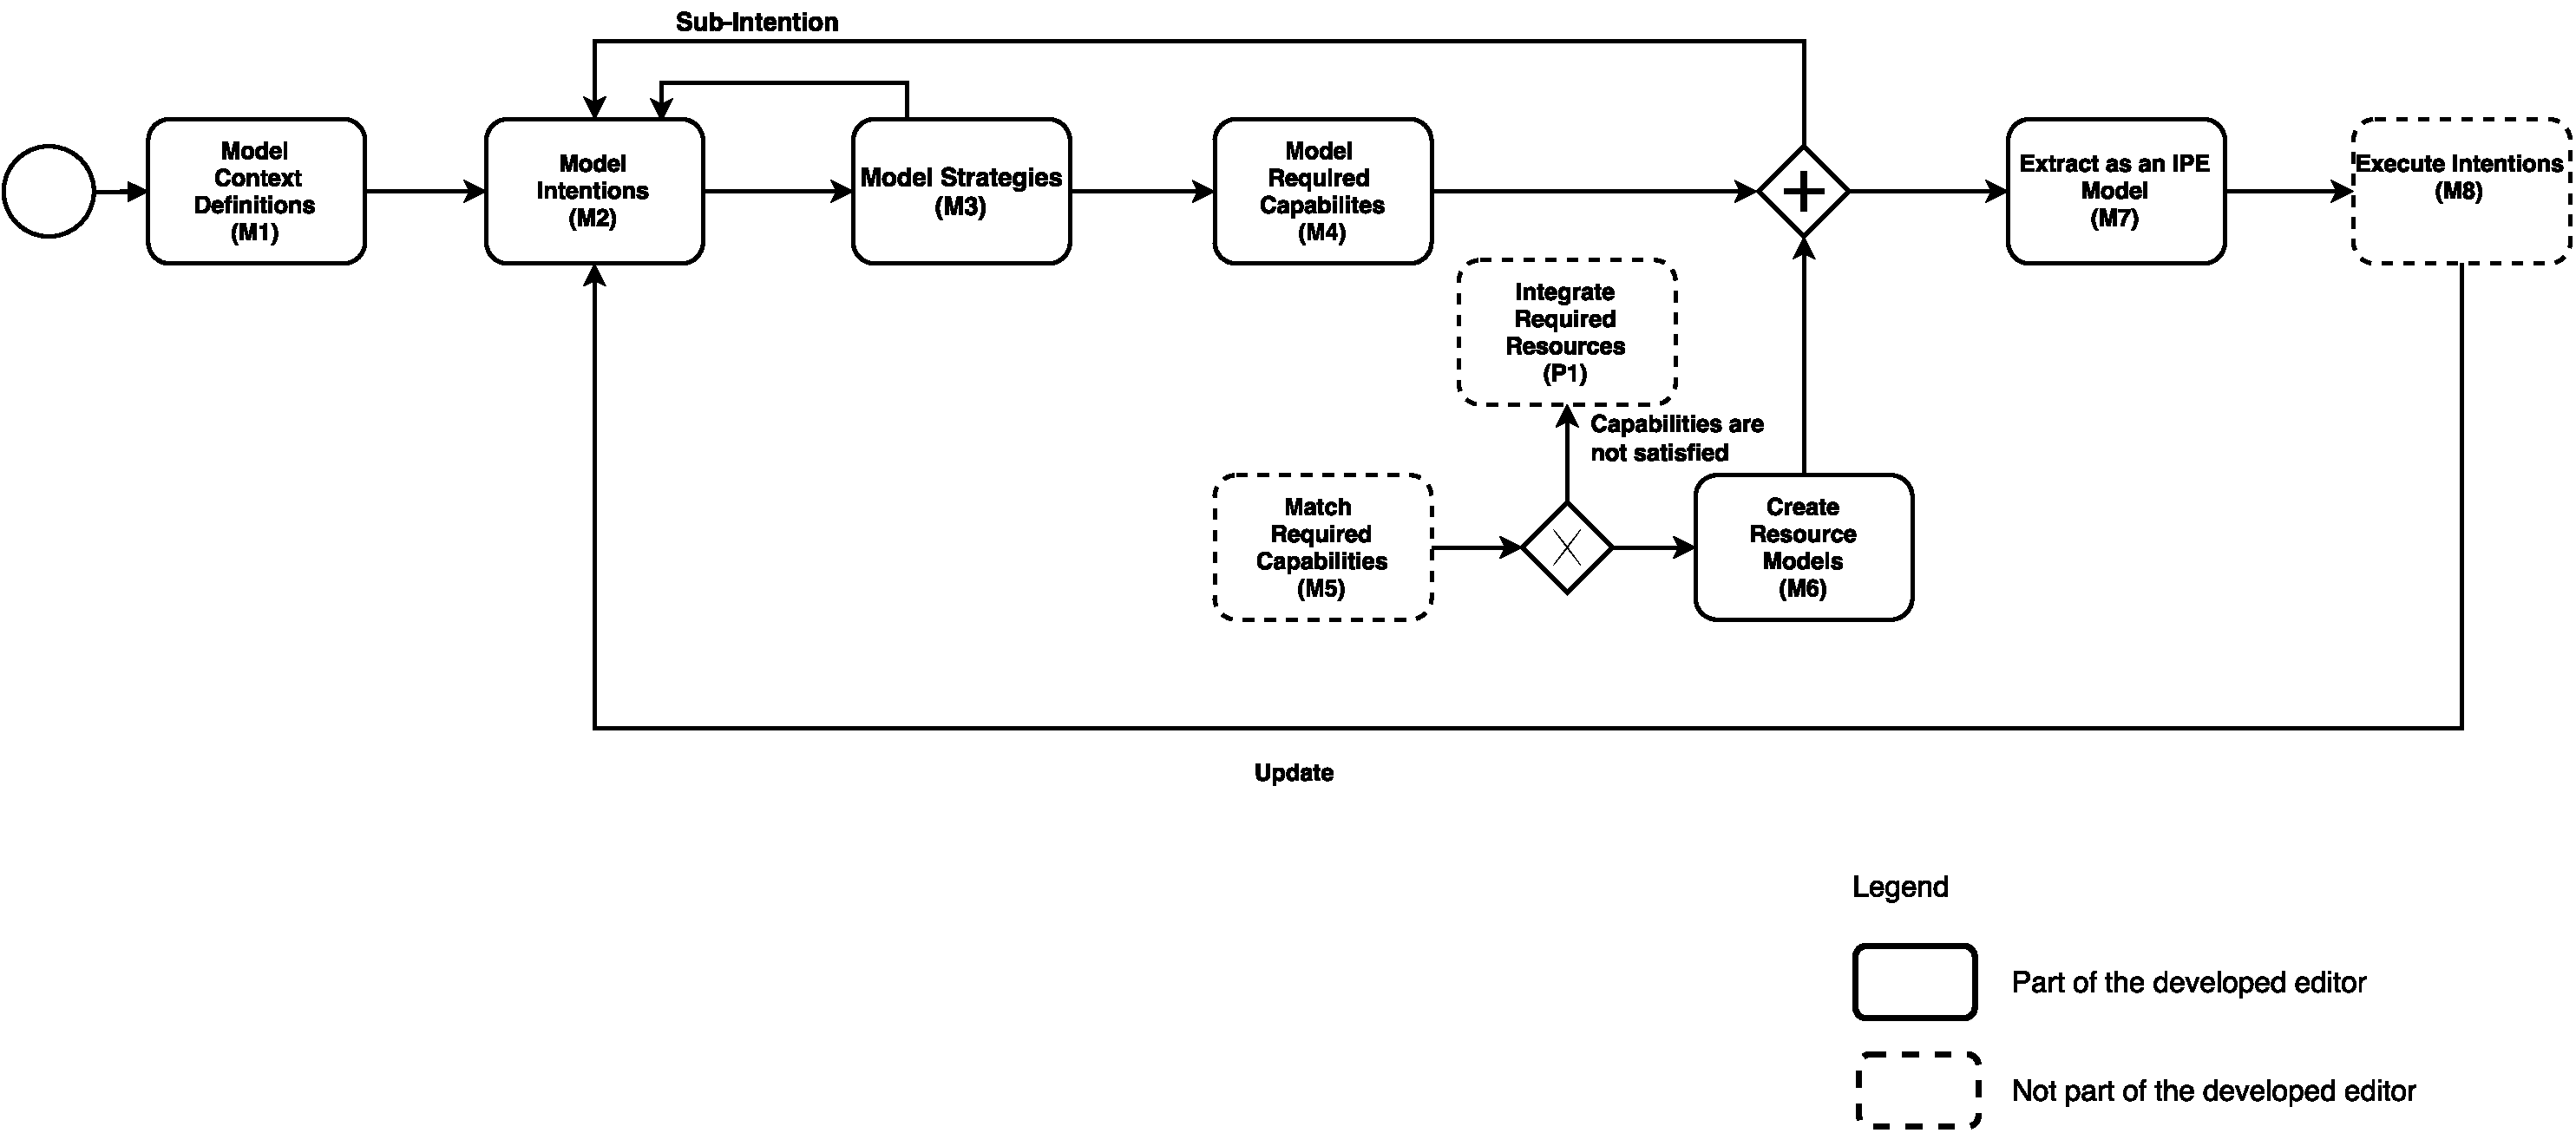
\includegraphics[width=\textwidth]{processmodeling.pdf}
	\caption{Process Modeling Diagram}
	\label{fig:processdiagram}
\end{figure}

%%%%%%%%%%%%%%%%%%%%%%%%%%%%%%%%%%%%%%%%%%%%%%%%%%%%%%%%%%%%%%%%%%%%%%%%%
\subsection{Entity Representation}
%%%%%%%%%%%%%%%%%%%%%%%%%%%%%%%%%%%%%%%%%%%%%%%%%%%%%%%%%%%%%%%%%%%%%%%%%

 The conceptual entity model of goals is shown in the \ref{fig:metamodel}. This model shows that top level goal is refined into sub-goals. A goal can be achieved through a strategy which is a plan of action designed to meet a goal. It also describes a set of interrelated resources which work together to achieve a collective goal. As reported by Sungur et al. \cite{Sungur2014a}, the concept of IPE provides an agent-based approach i.e., human performers are considered as agents who execute the processes autonomously. Based on the approach \cite{Sungur2014a} we provide a goal-oriented approach based on goals.

 Organizational Process Modeling  has \textit{Resources} which are used to achieve the goals. Organizational Process Modeling is Resource-centric approach as they support processes by providing required resources and thrives to successfully execute the processes by using qualified autonomous agents, i.e., actors under certain \textit{context definitions}.  Resources can be anything like people, IT tools, data that are used to accomplish the objectives.Emerging goals can result in the requirement of new capabilities, i.e., resources. A more specific type of resource is the type \textit{Actor}, which typically refers to human performers who autonomously and collaboratively conclude an organizational process using other available Organizational Process Modeling Resources.Actors work towards the goals defined in the process. Resource models are optional to make precise definitions of resources needed.

 In Sungur et al \cite{Sungur2014a} work, the concept of \textit{Informal Process Support Model} IPSM has been introduced which is to make use of existing knowledge of human performers. Here the initial creator of the model is experienced human performers. Based on their experience, they add relevant  resources of an informal process. Each of the resources has inter relationships among the resources themselves. The models are generated at runtime based on the interactions and activities of corresponding human performers. 

 An informal process targets for accomplishment of a goal. The goals can be refined by defining sub-goals, which can be defined recursively as independent informal processes. The goal-based approach enables describing processes declaratively, i.e., without describing \textit{how} the intention is achieved, and providing only information about \textit{what} is achieved. Thus, to avoid predefined business logic in the representations of informal processes. 

 Each informal process starts from an initial context, i.e., \textit{IPE Context} and aims to achieve a goal. After accomplishing the goal, there is a resulting context called as final context. Each Resource can be related to another Resource in the context of an informal process using predefined or custom \textit{Relationships}.
 
 \begin{figure}
 	\centering
 	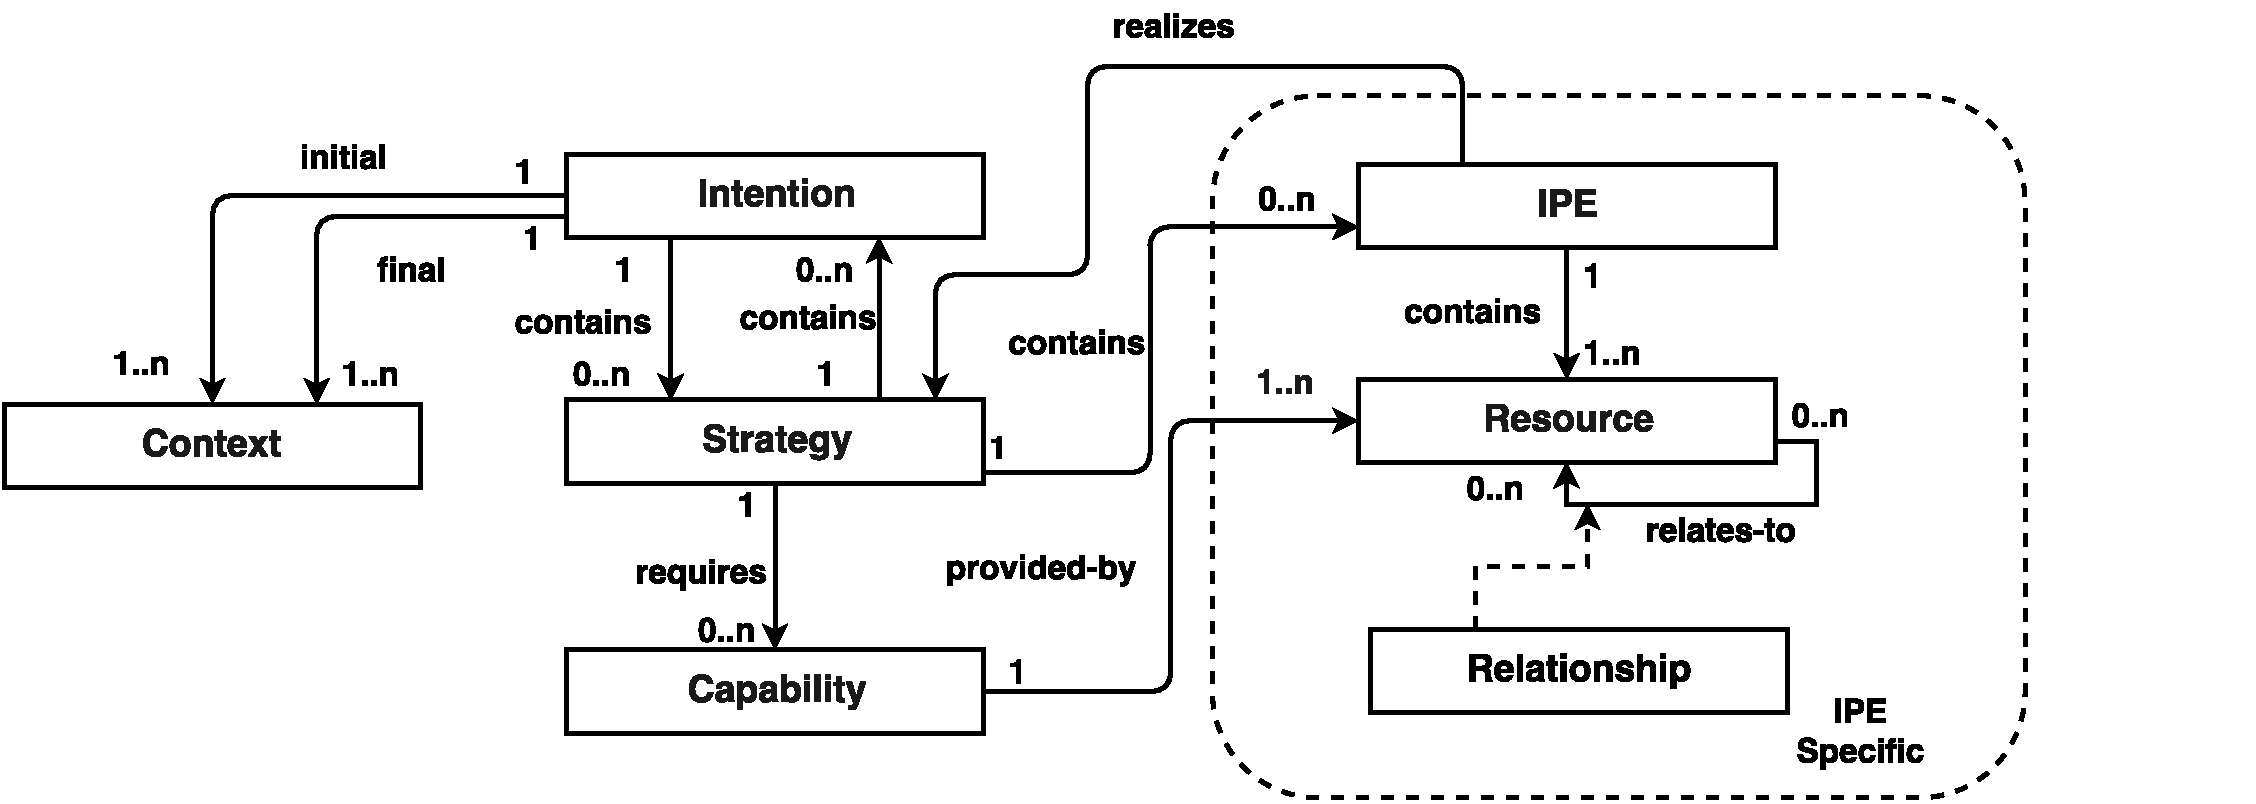
\includegraphics[width=\textwidth]{entity.pdf}
 	\caption{Organizational Modelling Meta-Model}
 	\label{fig:metamodel}
 \end{figure}
 

